\chapter{Thực nghiệm}
Với mục tiêu tìm hiểu và giải quyết bài toán phân loại thực khuẩn với dữ liệu đầu vào là contig, nhóm sinh viên thực hiện các thử nghiệm và đánh giá tương tự với nhóm tác giả DeePhage. Chương này trình bày phương pháp xây dựng bộ dữ liệu, các chỉ số đánh giá, kịch bản và kết quả thực nghiệm.

\section{ Xây dựng bộ dữ liệu}
\subsection{ Xử lý nhãn }
Sau khi tìm hiểu các bài báo, nhóm sinh viên thực hiện xây dựng bộ dữ liệu mới dựa trên 2 bộ dữ liệu được sử dụng trong bài báo DeepPL và DeePhage. Nhãn $y$ của bản ghi $X$ được nhóm sinh viên xử lý như sau:
\begin{enumerate}
    \item Nếu $X \in DeePhage \Rightarrow y = y_{DeePhage}$ 
    \item Nếu $X \in DeepPL \Rightarrow y = y_{DeepPL}$
    \item Nếu $X \in DeePhage \cap DeepPL \Rightarrow y = y_{DeePhage}$
\end{enumerate}

\section{Kịch bản thực nghiệm}\label{ kịch bản thực nghiệm}
Để tiến hành các thực nghiệm, nhóm sinh viên chọn 2 mô hình là DeePhage và XGBoost. Nhận thấy DeePhage là công cụ  hài hòa trong nhóm các phương pháp dựa trên học sâu khi mà hiệu suất phân loại tốt đồng thời có thời gian huấn luyện nhanh, nhóm sinh viên quyết định chọn DeePhage là công cụ tiêu chuẩn trong các thực nghiệm. Ngoài ra, do cần 1 mô hình đủ mạnh để có thể có hiệu suất phân loại tốt cũng như nhanh trong quá trình huấn luyện, nhóm quyết định chọn XGBoost là mô hình được sử dụng để trực tiếp so sánh với DeePhage.

\section{Các chỉ số đánh giá}
Để đánh giá 1 cách toàn diện hiệu suất phân loại của mô hình chứ không chỉ tập trung vào nhãn 1, nhóm sinh viên sử dụng các chỉ số sau:
\begin{itemize}
    \item Accuracy: sử dụng để do lường hiệu suất phân loại chung của mô hình trên 2 nhãn.
    \item Sensitivity: sử dụng để đo lường dộ phủ của mô hình trên nhãn 1.
    \item Specificity: sử dụng để đo lường độ phủ của mô hình trên nhãn 0.
\end{itemize}

\section{Kết quả}
\subsection{Kết quả thực nghiệm với PhageAI}
Trong thí nghiệm này, chúng tôi thực hiện thử nghiệm các thuật toán học máy trong bài báo PhageAI với bộ dữ liệu mới. Các mô hình đều sử dụng BayesianSearch để tối ưu lựa chọn các bộ tham số tốt nhất. Riêng với thuật toán SVM, chúng tôi sử dụng bộ tham số đã được tác giả công bố trong bài báo.
\begin{table}[ht]
\footnotesize
\centering
\begin{tabular}{|l|c|c|c|}
\hline
\textbf{Model} & \textbf{Accuracy} & \textbf{Sensitivity (Class 1)} & \textbf{Specificity (Class 0)} \\
\hline
GaussianNB & 0.649 & 0.780 & 0.365 \\
SGDClassifier & 0.864 & 0.861 & 0.869 \\
MLPClassifier & 0.901 & 0.946 & 0.803 \\
RandomForestClassifier & 0.928 & \textbf{0.963} & 0.854 \\
SVC & 0.901 & 0.882 & \textbf{0.942} \\
KNeighborsClassifier & 0.910 & 0.909 & 0.912 \\
GradientBoostingClassifier & 0.930 & 0.951 & 0.882 \\
XGBoost & \textbf{0.936} & 0.959 & 0.883 \\
LightGBM & 0.933 & 0.951 & 0.878 \\
CatBoost & 0.931 & 0.953 & 0.870 \\
\hline
\end{tabular}
\caption{Kết quả so sánh các thuật toán học máy theo Accuracy, Sensitivity và Specificity trên bộ dữ liệu kết hợp.}
\label{tab:model_comparison}
\end{table}

Dựa trên kết quả Bảng \ref{tab:model_comparison}, có thể thấy rằng các mô hình thuộc nhóm ensemble learning, đặc biệt là các thuật toán Boosting như XGBoost, LightGBM, CatBoost và GradientBoostingClassifier, đều cho hiệu suất rất cao trên cả ba chỉ số: Accuracy, Sensitivity và Specificity. Trong đó, XGBoost đạt Accuracy cao nhất (0.936), đồng thời duy trì mức Sensitivity (0.959) và Specificity (0.883) rất cân bằng, cho thấy khả năng phân biệt tốt giữa hai lớp.

RandomForestClassifier cũng thể hiện hiệu quả cao với Accuracy 0.928, tuy nhiên có phần thiên lệch hơn về Sensitivity (0.963) so với Specificity (0.854), nghĩa là mô hình có xu hướng nhạy hơn với lớp dương (Class 1).

Ở nhóm mô hình cơ bản hơn như GaussianNB và SGDClassifier, kết quả không thực sự khả quan. Đặc biệt, GaussianNB cho Specificity chỉ ở mức 0.365, cho thấy mô hình này khó phân biệt được lớp âm (Class 0), mặc dù có Sensitivity tương đối tốt (0.780). Điều này thường xảy ra khi dữ liệu không phù hợp với giả định phân phối chuẩn của Naive Bayes.

MLPClassifier và SVC đều có Accuracy trên 0.9, nhưng mỗi mô hình có thiên hướng riêng: MLPClassifier nghiêng về phát hiện Class 1 (Sensitivity cao 0.946), trong khi SVC lại rất mạnh trong việc nhận diện Class 0 (Specificity 0.942).

Tổng thể, như vậy khác với tập dữ liệu của bài báo với SVC cho kết quả tốt nhất thì trong thực nghiệm này, các mô hình Boosting như XGBoost và GradientBoostingClassifier tỏ ra vượt trội về độ chính xác và cân bằng giữa các chỉ số, phù hợp với các bài toán phân loại nhị phân có yêu cầu cao về độ tin cậy. 
\subsection{So sánh hiệu suất phân loại giữa DeePhage và XGBoost trên bộ dữ liệu xây dựng}

\begin{figure}[H]
    \centering
    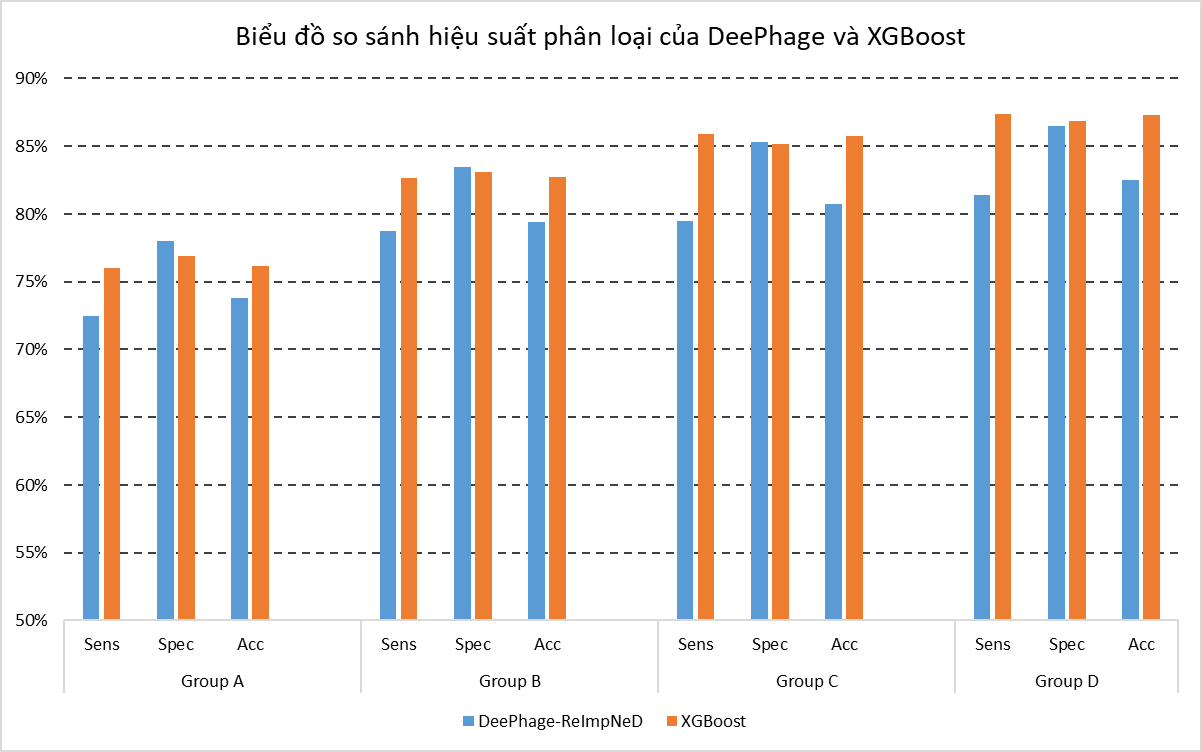
\includegraphics[width=1\linewidth]{figures/result_deephage_vs_xgboost.png}
    \caption{Kết quả hiệu suất phân loại của mô hình XGBoost trên tập dữ liệu xây dựng.}
    \label{fig:result_2}
\end{figure}

Hình \ref{fig:result_2} là biểu đồ so sánh hiệu suất phân loại của DeePhage và XGBoost trên tập dữ liệu mà nhóm sinh viên xây dựng. Có thể thấy, DeePhage cho kết quả tốt hơn 1 chút, khoảng từ 2\% - 5\% khi hơn XGBoost ở 2 chỉ số Sensitivity và Accuracy. Nghĩa là DeePhage cho khả năng nhận diện nhãn 1 và độ chính xác tổng thể cao hơn. Với chỉ số Specificity, XGBoost cho kết quả tốt hơn khoảng 5\%, nghĩa là khả năng nhận diễn nhãn 0 của XGBoost tốt hơn DeePhage.

